\documentclass[12pt]{article}
\usepackage{bbm}
\usepackage{amsmath}
\usepackage[colorlinks=true]{hyperref}
\usepackage{enumitem}
\usepackage[a4paper, total={6in, 9in}]{geometry}
\usepackage{tikz}

\begin{document}

\title{COS 516: Final Project Report\\
\emph{Proving the Correctness of the Normal Equations with Dafny}} %Replace X with homework number, Y with problem number.
\author{Samuel Sanft}
\date{\today}
\maketitle

\section*{Honor Statement}
This assignment represents my own work in accordance with university policy.

\section{Introduction \& Overview}
The normal equations refer to the following equation and its associated solution ($A \in \mathbbm{R}^{m \times n}, b \in \mathbbm{R}^m, x \in \mathbbm{R}^n$):
\begin{align*}
A^T A x &= A^T b \\
x &= (A^T A)^{-1} A^T b
\end{align*}

This solution for $x$ (a unique solution exists when $A^T A$ is invertible, or when the columns of $A$ are linearly independent), is the optimal solution to the following ordinary least squares (OLS) optimization problem (let $||\cdot||$ be the euclidean or 2-norm):
$$\min_x ||Ax - b||^2$$
See \hyperref[sec:mathproof]{Appendix 5.1} for a complete mathematical proof.

The goal of this project is to formalize this problem and provide a machine-checked proof that the solution of the normal equations is equivalent to an optimal solution of the OLS optimization problem using Dafny. This goal can be split into two parts:
\begin{itemize}
\item specifying the problem and it's solution, which requires an implementation of linear algebraic types (matrices and vectors) and operations (matrix and vector arithmetic), and
\item constructing a proof to show that the solution to the normal equations is optimal, which requires first writing proofs about known properties of linear algebraic operations.
\end{itemize}

\section{Project Tasks}
\subsection{Implementation}
\subsubsection{Data Types}
The first step of the implementation was defining abstract data types for matrices and vectors. Dafny differentiates between functions and methods. Methods may have side effects but may not be used in expressions. Functions may not have side effects but may be used in expressions. Because of the need to use linear algebraic operations in order to define the OLS optimization problem, I opted to implement all of the operations using functions. This decision informed how I chose to implement the data types. Because my operations can not have side effects (they must be purely functional), this meant that I couldn't use arrays or other data types that manipulate data in the heap. Instead I opted to implement the data types using functional data structures.

The \verb|Matrix| type is defined as a tuple, consisting of a two-dimensional sequence of real numbers and two integers, representing the dimensions of the matrix. The module also contains the functions \verb|matNumRows|, \verb|matNumCols|, and \verb|matGet|, which return the number of rows in a matrix, the number of columns in a matrix, or a given entry in a matrix. The function signatures, with their specified  requirements and guarantees are given:

\begin{verbatim}
function matNumRows (mat : Matrix) : int
ensures 0 <= matNumRows (mat)

function matNumCols (mat : Matrix) : int
ensures 0 <= matNumCols (mat)

function matGet (mat : Matrix, i : int, j : int) : real
requires 0 <= i < matNumRows (mat)
requires 0 <= j < matNumCols (mat)
\end{verbatim}

The \verb|Vector| type is defined inductively, either as a sequence of real numbers, or as a specified row or column of a matrix. The module then has two functions that return a column or a row of a matrix as a vector, as well as functions to return the length of a vector and an entry within a vector. The function signatures are given below:

\begin{verbatim}
function matGetRow (mat : Matrix, i : int) : (res : Vector)
requires 0 <= i < matNumRows (mat)
ensures vecLength (res) == matNumCols (mat)

function matGetCol (mat : Matrix, i : int) : (res : Vector)
requires 0 <= i < matNumCols (mat)
ensures vecLength (res) == matNumRows (mat)

function vecLength (vec : Vector) : int
ensures 0 <= vecLength(vec)

function vecGet (vec : Vector, i : int) : real
requires 0 <= i < vecLength (vec)
\end{verbatim}

The following predicate was also defined, to test the equality of two equally sized vectors:

\begin{verbatim}
predicate vecEquals (vec1 : Vector, vec2 : Vector)
requires vecLength (vec1) == vecLength (vec2)
{
    forall i | 0 <= i < vecLength (vec1) ::
        vecGet (vec1, i) == vecGet (vec2, i)
}
\end{verbatim}

\subsubsection{Vector Arithmetic}
The following operations were implemented for vector arithmetic (for complete signatures, requirements, and guarantees, see \hyperref[sec:vectorsigs]{Appendix 5.2.1}):
\begin{itemize}
\item Dot-Product
\item Squared Norm
\item Vector Addition
\item Vector Subtraction
\item Vector Scaling
\end{itemize}

These functions were all defined recursively instead of using loops. As an example, the code for \verb|vecDotProd| is given below. The functions only access the \verb|Vector| data structure through the functions defined in the vector module, meaning that the implementation of the \verb|Vector| abstract data type can be rewritten without having to rewrite any of the arithmetic operations. Also, because the functions are written recursively, it is easier to reason about them, as there is no need for loop invariants and proofs can be done inductively, which will be seen in \hyperref[sec:proofs]{Section 2.2 Proofs}.

\begin{verbatim}
function vecDotProd (vec1 : Vector, vec2 : Vector) : real
requires vecLength (vec1) == vecLength (vec2)
{
    vecDotProdAux (vec1, vec2, 0)
}

function vecDotProdAux (vec1 : Vector, vec2 : Vector, i : int) : real
requires vecLength (vec1) == vecLength (vec2)
requires 0 <= i <= vecLength (vec1)
decreases vecLength (vec1) - i
{
    if i == vecLength (vec1)
    then 0.0
    else vecGet (vec1, i) * vecGet (vec2, i) +
        vecDotProdAux (vec1, vec2, i + 1)
}
\end{verbatim}

\subsubsection{Matrix Arithmetic}
The following operations were implemented for matrix arithmetic (see \hyperref[sec:matrixsigs]{Appendix 5.2.2} for signatures, requirements, and guarantees):
\begin{itemize}
\item Matrix-Vector Multiplication
\item Matrix-Matrix Multiplication
\end{itemize}

Additionally, the following predicates were implemented for:
\begin{itemize}
\item checking the equality of two matrices
\item checking whether two matrices are transposes
\item checking whether a matrix is symmetric
\item checking whether a matrix is the identity
\item checking whether two matrices are inverses
\end{itemize}

The multiplication functions are implemented recursively and use the \verb|vecDotProd| function. The predicates are all useful for reasoning about linear algebraic operations and writing related proofs.

\subsection{Proofs}
\label{sec:proofs}
Note: Let $\langle \cdot, \cdot \rangle$ be the notation for the dot-product of two vectors.

Proofs about the basic properties of all of the implemented operations were written as lemmas in the Dafny language. Some lemmas were able to be proven automatically with little to no manual input. For example, the following lemma about the transitivity of vector addition (for any vectors $x, y, z$ of equal length, $(x + y) + z = x + (y + z)$) required no function body in order to be verified:

\begin{verbatim}
lemma vecAddTransitive (vec1 : Vector, vec2 : Vector, vec3 : Vector)
requires vecLength (vec1) == vecLength (vec2)
requires vecLength (vec1) == vecLength (vec3)
ensures vecEquals (
    vecAdd (vecAdd (vec1, vec2), vec3),
    vecAdd (vec1, vecAdd (vec2, vec3))
)
\end{verbatim}

For functions that were implemented using an auxiliary recursive function, for example \verb|vecDotProd| and \verb|vecDotProdAux|, an extra lemma reasoning about the auxiliary function was usually necessary. For example, in order to show that the dot product is distributive with addition (for any vectors $x, y, z$ of equal length, $\langle x, y + z \rangle = \langle x, y \rangle + \langle x, z \rangle$), first a lemma is defined that shows that the auxiliary method is distributive with addition:

\begin{verbatim}
lemma vecDotProdAuxDist (vec1 : Vector, vec2 : Vector,
                         vec3 : Vector, i : int)
requires vecLength (vec1) == vecLength (vec2)
requires vecLength (vec1) == vecLength (vec3)
requires 0 <= i <= vecLength (vec1)
ensures vecDotProdAux (vec1, vecAdd (vec2, vec3), i) == 
    vecDotProdAux (vec1, vec2, i) + vecDotProdAux (vec1, vec3, i)
decreases vecLength (vec1) - i
{}

lemma vecDotProdDistR (vec1 : Vector, vec2 : Vector, vec3 : Vector)
requires vecLength (vec1) == vecLength (vec2)
requires vecLength (vec1) == vecLength (vec3)
ensures vecDotProd (vec1, vecAdd (vec2, vec3)) == 
    vecDotProd (vec1, vec2) + vecDotProd (vec1, vec3)
{
    vecDotProdAuxDist (vec1, vec2, vec3, 0);
}
\end{verbatim}

\verb|vecDotProdAuxDist| proves the guarantee inductively on the length of the vectors thanks to the statement \verb|decreases vecLength (vec1) - i|. This is the only hint the solver needs in order to prove the lemma. Following the auxiliary lemma's verification, the main lemma can easily be proven with an application of the auxiliary where $i = 0$.

Some of the lemmas were more difficult to prove, requiring a number of simpler lemmas to be proven first. For example, the lemma \verb|vecNormDistSub| provides the following guarantee, for any vectors \verb|vec1| and \verb|vec2| of equal length:
\begin{verbatim}
vecNormSq (vecSub (vec1, vec2)) == 
    vecNormSq (vec1) - 2.0 * vecDotProd (vec1, vec2) + vecNormSq (vec2)
\end{verbatim}
In mathematical terms, for any vectors $v_1, v_2$ of equal length, $||v_1 - v_2||^2 = ||v_1||^2 - \langle v_1, v_2 \rangle + ||v_2||^2$. This lemma required 12 seperate lemmas to be verified first. The complete dependency graph is shown in \autoref{fig:dep-graph}.

\begin{figure}[h]
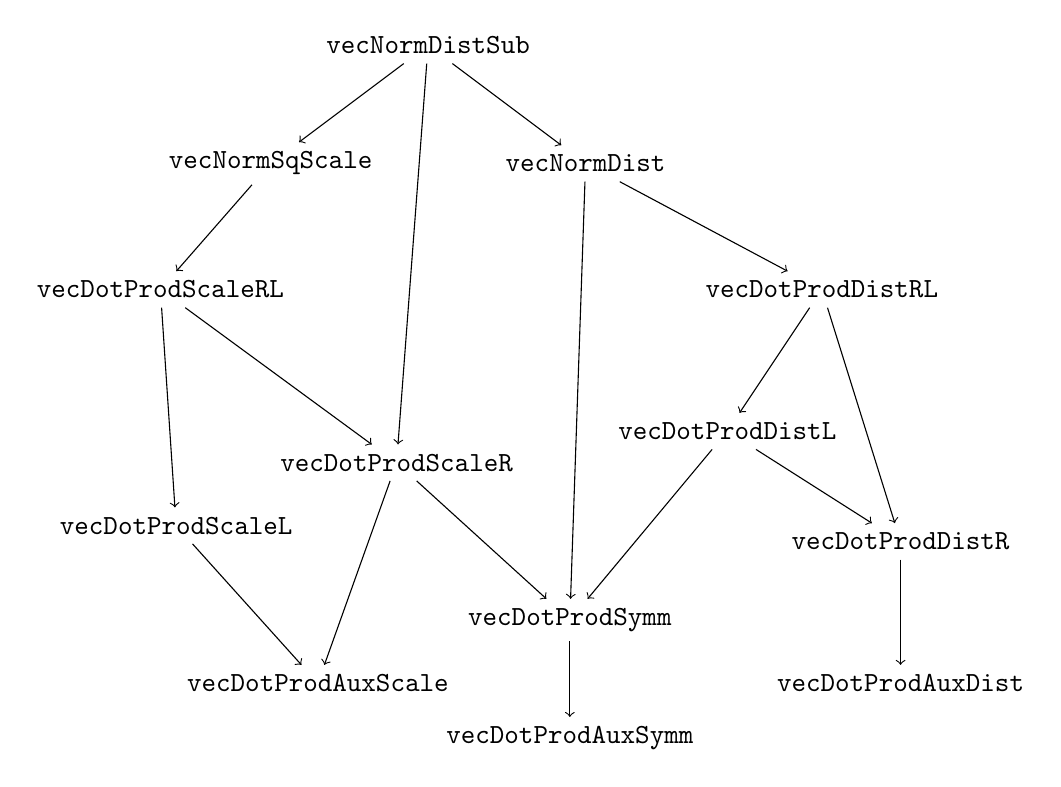
\begin{tikzpicture}
\node (v0) at (6,-1.8) {\verb|vecDotProdAuxDist|};
\node (v1) at (-1.4,-1.8) {\verb|vecDotProdAuxScale|};
\node (v2) at (3.8,1.4) {\verb|vecDotProdDistL|};
\node (v3) at (6,0) {\verb|vecDotProdDistR|};
\node (v4) at (5,3.2) {\verb|vecDotProdDistRL|};
\node (v5) at (-3.2,0.2) {\verb|vecDotProdScaleL|};
\node (v6) at (-0.4,1) {\verb|vecDotProdScaleR|};
\node (v7) at (-3.4,3.2) {\verb|vecDotProdScaleRL|};
\node (v8) at (1.8,-1) {\verb|vecDotProdSymm|};
\node (v9) at (2.,4.8) {\verb|vecNormDist|};
\node (v10) at (0,6.3) {\verb|vecNormDistSub|};
\node (v11) at (-2,4.8) {\verb|vecNormSqScale|};
\node (v12) at (1.8, -2.5) {\verb|vecDotProdAuxSymm|};
\draw [->] (v2) edge (v3);
\draw [->] (v2) edge (v8);
\draw [->] (v3) edge (v0);
\draw [->] (v4) edge (v2);
\draw [->] (v4) edge (v3);
\draw [->] (v5) edge (v1);
\draw [->] (v6) edge (v1);
\draw [->] (v6) edge (v8);
\draw [->] (v7) edge (v5);
\draw [->] (v7) edge (v6);
\draw [->] (v9) edge (v4);
\draw [->] (v9) edge (v8);
\draw [->] (v10) edge (v6);
\draw [->] (v10) edge (v9);
\draw [->] (v10) edge (v11);
\draw [->] (v11) edge (v7);
\draw [->] (v8) edge (v12);
\end{tikzpicture}
\caption{Lemma dependencies}
\label{fig:dep-graph}
\centering
\end{figure}

The most difficult lemma to prove was \verb|dotProdTr|, which has the following guarantee for the appropriately shaped matrix and vectors \verb|mat|, \verb|vec1|, \verb|vec2|:

\begin{verbatim}
vecDotProd (matVecMult (mat, vec1), vec2) == 
    vecDotProd (vec1, matVecMult (matTr (mat), vec2))
\end{verbatim}

In mathematical terms, for any $A \in \mathbbm{R}^{m \times n}, v_1 \in \mathbbm{R}^n, v_2 \in \mathbbm{R}^m$, $\langle Av_1, v_2 \rangle = \langle v_1, A^T v_2 \rangle$. This lemma was very challenging to prove inductively, because the order of operations is different for the left and right hand sides of the equation. Ultimately, this lemma required a second version of the matrix-vector multiplication operation to be implemented, which computes the result in column-major instead of row-major order. After proving that the two multiplication functions are equivalent, both were used in order to prove the lemma.

After proving a sufficient number of lemmas about the basic properties of the implemented linear algebraic operations, it became possible to prove that the solution to the normal equations is an optimal solution to the OLS problem. For a rough outline of the proof used in mathematical terms, refer to \hyperref[sec:mathproof]{Appendix 5.1}. The final lemma depended on 9 different lemmas (each of which had their own dependencies) and used 24 lemma applications in its body. The proof involved applying a series of rewrites to show that (let $x^* = (A^T A)^{-1} A^T b$, let $x$ be any vector with the appropriate length):
\begin{align*}
||Ax^* - b||^2 &\le ||Ax - b||^2 \\
&\downarrow \\
-\langle Ax^*, b \rangle + ||b||^2 &\le ||Ax - Ax^*||^2 - \langle Ax^*, b \rangle + ||b||^2 \\
0 &\le ||Ax - Ax^*||^2
\end{align*}

One remark worth mentioning, is that no function for finding the inverse of a matrix was implemented, but rather a predicate that checks whether two matrices are inverses. This means if a user wants to call the \verb|normalEquations| method, which returns a solution to the normal equations, they must provide $(A^T A)^{-1}$ as an argument, as well as $A$ and $b$ (the function verifies that this is a valid inverse using the predicate). While unideal, this does mean that the program doesn't have to reason about whether or not a unique solution exists, because a unique solution exists if and only if $A^T A$ is invertible (which the user must demonstrate by providing a valid inverse).

\section{Results \& Discussion}
Ultimately I was able to complete all of the proofs so that they could be verified by Dafny's solver. I consider the results of the project to be successful, as I was able to achieve the original goal laid out for the project. With more time to work on the project I would've liked to have fully implemented matrix inverses, although I suspect that would've required a significant amount of engineering effort, both for the implementation itself and for the associated proofs. Should I continue the project in the future, that would be my next step. Other further work could also include proving optimal solutions for related optimization problems such as the ridge regression problem, or writing more efficient implementations of the \verb|Vector| and \verb|Matrix| abstract data types.

The final project had a little more than 300 lines of code for the implementation of the data types and all of the associated operations and around 700 lines of code for the final proof and all of the associated lemmas. This means that there were roughly 2 lines of proofs for every line of code for the implementation. In terms of total effort I would say that the proofs were certainly more difficult to write and I would estimate that I spent maybe 4-5 hours of writing proofs for every hour I spent working on the implementation.

I would say that writing the code in Dafny made verifying the proofs much easier compared to using a traditional proof-assistant like Coq. Anecdotally, in my experience with Coq, the ratio of time spent working on proofs compared to on implementations has often been around 10:1. It was very helpful that I could simply tell Dafny to verify a lemma by induction by providing a \verb|decreases| statement, without having to actually reason about the individual cases. Using Dafny to write a mostly functional program was also interesting, as a lot of Dafny's tools are geared towards imperative programming. For example, the Dafny reference manual (\href{https://dafny.org/dafny/DafnyRef/DafnyRef}{link}) has relatively little information about inductive data types, recursion or higher-order functions. Additionally, Dafny can not be used to generate code in languages like OCaml or Haskell, unlike Coq, as it currently only allows compilation into imperative languages (see \href{https://dafny.org/latest/DafnyRef/DafnyRef#sec-dafny-translate}{User Manual} for a complete list of supported languages). Based on my experience with this project, I would say it's definitely possible to write verified functional programs in Dafny, but certain restraints may apply due to Dafny's limitations, and if efficient performance is desired, a tool like Coq may be better suited.

\section{Conclusion}
In conclusion, this project contains implementations for verified abstract data types for vectors and matrices as well as verified functions to perform vector and matrix arithmetic. It also includes verified proofs to show that many mathematical properties of linear algebra hold under this implementation. Finally it has a verified proof that shows that the solution to the normal equations, $x = (A^T A)^{-1} A^T b$, is an optimal solution to the OLS optimization problem. I found working on this project to be very enjoyable and learned a lot about Dafny, and it's capabilities and limitations, as well as verification in general. I would look forward to completing similar verified programs in the future, whether with Dafny or with other similar tools.

\section{Appendix}
\subsection{Proof of Optimality of Normal Equations}
\label{sec:mathproof}
In this section, a proof is provided that the solution to the normal equations is an optimal solution to the OLS problem. The proof roughly matches the structure of the proof that is written in Dafny. Since the squared euclidean norm is a convex function, this is normally done by showing that the solution to the normal equations satisfies the first-order optimality conditions for the OLS problem. However, in order to verify the proof in Dafny without implementing symbolic or automatic differentiation, it was necessary to find a proof that did not require differentiation. That proof is given here.

In order to show that the normal equations provide an optimal solution to the OLS problem, it is sufficient to show (let $x^* := (A^T A)^{-1} A^T b$):
$$\forall x, ||Ax^* - b||^2 \le ||Ax - b||^2$$

\subsubsection{Lemma 1}
\begin{align*}
||Ax^*||^2 &= -\langle Ax^*, b \rangle \\
\cline{1 - 2}
||Ax^*||^2 &= \langle Ax^*, Ax^* \rangle \\
 &= \langle x^*, A^T Ax^* \rangle \\
 &= \langle x^*, A^T A (A^T A)^{-1} A^T b \rangle \\
 &= \langle x^*, A^T b \rangle \\
 &= \langle Ax^*, b \rangle
\end{align*}

\subsubsection{Lemma 2}
Using Lemma 1:
\begin{align*}
||Ax^* - b||^2 &= -\langle Ax^*, b \rangle + ||b||^2 \\
\cline{1 - 2}
||Ax^* - b||^2 &= ||Ax^*||^2 - 2 \langle Ax^*, b \rangle + ||b||^2 \\
 &= \langle Ax^*, b \rangle - 2 \langle Ax^*, b \rangle + ||b||^2 \\
 &= -\langle Ax^*, b \rangle + ||b||^2
\end{align*}

\subsubsection{Lemma 3}
Using Lemma 1:
\begin{align*}
||Ax - b||^2 &= ||Ax - Ax^*||^2 - \langle Ax^*, b \rangle + ||b||^2 \\
\cline{1 - 2}
||Ax - b||^2 &= ||Ax||^2 - 2 \langle Ax, b \rangle + ||b||^2 \\
 &= ||Ax||^2 - 2 \langle A (A^T A)^{-1} A^T A x, b \rangle + ||b||^2 \\
 &= ||Ax||^2 - 2 \langle Ax, A (A^T A)^{-1} A^T b \rangle + ||b||^2 \\
 &= ||Ax||^2 - 2 \langle Ax, Ax^* \rangle + ||Ax^*||^2 - ||Ax^*||^2 + ||b||^2 \\
 &= ||Ax - Ax^*||^2 - ||Ax^*||^2 + ||b||^2 \\
 &= ||Ax - Ax^*||^2 - \langle Ax^*, b \rangle + ||b||^2
\end{align*}

\subsubsection{Proof}
Now the original inequality can be demonstrated, using Lemmas 2 and 3 and the fact that the euclidean norm is always nonnegative:
\begin{align*}
||Ax^* - b||^2 &\le ||Ax - b||^2 \\
-\langle Ax^*, b \rangle + ||b||^2 &\le ||Ax - Ax^*||^2 - \langle Ax^*, b \rangle + ||b||^2 \\
0 &\le ||Ax - Ax^*||^2
\end{align*}

\subsection{Code}
\subsubsection{Vector Function Signatures}
\label{sec:vectorsigs}
\begin{verbatim}
function vecDotProd (vec1 : Vector, vec2 : Vector) : real
requires vecLength (vec1) == vecLength (vec2)

function vecNormSq(vec : Vector) : real

function vecAdd (vec1 : Vector, vec2 : Vector) : (res : Vector)
requires vecLength (vec1) == vecLength (vec2)
ensures vecLength (res) == vecLength (vec1)
ensures forall i | 0 <= i < vecLength (res) ::
    vecGet (res, i) == vecGet (vec1, i) + vecGet (vec2, i)

function vecSub (vec1 : Vector, vec2 : Vector) : (res : Vector)
requires vecLength (vec1) == vecLength (vec2)
ensures vecLength (res) == vecLength (vec1)
ensures forall i | 0 <= i < vecLength (res) ::
    vecGet (res, i) == vecGet (vec1, i) - vecGet (vec2, i)

function vecScale (alpha : real, vec : Vector) : (res : Vector)
ensures vecLength (res) == vecLength (vec)
ensures forall i | 0 <= i < vecLength (vec) ::
    vecGet (res, i) == alpha * vecGet (vec, i)
\end{verbatim}

\subsubsection{Matrix Function Signatures and Predicates}
\label{sec:matrixsigs}
\begin{verbatim}
function matVecMult (mat : Matrix, vec : Vector) : (res : Vector)
requires matNumCols (mat) == vecLength (vec)
ensures vecLength (res) == matNumRows (mat)
ensures forall i | 0 <= i < matNumRows (mat) :: 
    vecGet (res, i) == vecDotProd (matGetRow (mat, i), vec)

function matMatMult (mat1 : Matrix, mat2 : Matrix) : (res : Matrix)
requires matNumCols (mat1) == matNumRows (mat2)
ensures matNumRows (mat1) == matNumRows (res)
ensures matNumCols (mat2) == matNumCols (res)
ensures forall i, j | 0 <= i < matNumRows (res) && 
    0 <= j < matNumCols (res) ::
    matGet (res, i, j) == vecDotProd (
        matGetRow (mat1, i), matGetCol (mat2, j)
    )

predicate matEquals (mat1 : Matrix, mat2 : Matrix)
requires matNumRows (mat1) == matNumRows (mat2)
requires matNumCols (mat1) == matNumCols (mat2)
{
    forall i | 0 <= i < matNumRows (mat1) ::
        vecEquals (matGetRow (mat1, i), matGetRow (mat2, i))
}

predicate matIsIdentity (mat : Matrix)
requires matNumRows (mat) == matNumCols (mat)
{
    forall i, j | 0 <= i < matNumRows (mat) && 
        0 <= j < matNumRows (mat) ::
        if i == j
        then matGet (mat, i, j) == 1.0 
        else matGet (mat, i, j) == 0.0
}

predicate matIsTranspose (mat1 : Matrix, mat2 : Matrix)
requires matNumRows (mat1) == matNumCols (mat2)
requires matNumCols (mat1) == matNumRows (mat2)
{
    forall i, j | 0 <= i < matNumRows (mat1) &&
        0 <= j < matNumCols (mat1) ::
        matGet (mat1, i, j) == matGet (mat2, j, i)
}

predicate matIsSymmetric (mat : Matrix)
requires matNumRows (mat) == matNumCols (mat)
{
    matIsTranspose (mat, mat)
}

predicate matIsInverse (mat1 : Matrix, mat2 : Matrix)
requires matNumRows (mat1) == matNumCols (mat1)
requires matNumRows (mat2) == matNumCols (mat2)
requires matNumRows (mat1) == matNumRows (mat2)
{
    matIsIdentity (matMatMult (mat1, mat2)) && 
        matIsIdentity (matMatMult (mat2, mat1))
}
\end{verbatim}

\end{document}
